\section{Introduction}
\label{section:introduction}

Safe driving is an important thing: a lot of incidents are due to 
distractions and fatigue. Therefore, it is important to keep the driver
alert and focused on driving a car or a truck. This is especially important 
during long distance and night drives. 

In this work we investigate a simple solution that constantly monitors 
the in-cabin driver's behavior and notifies it via sound alarms 
about the fatigue and distraction event occurrences. 

As part of the prototype implementation we have also implemented 
the simple backend that keeps track of GPS coordinates, stores 
short video clips (when fatigue and distraction is detected) and event types
in the database (although this part of the project is not exposed in the public 
Git repository).

The application are of this solution is broad: from improving the 
safety at mines to safety on city roads.

\section{CNN architecture}
\label{section:arch}

We have chosen a CNN network for the classification task with 3 convolutional 
layers (with 8, 16, and 32 feature maps), one flatten layer, one fully 
connected (or dense) regular NN layer, and output layer with two heads: one head for 
bounding box detection and one head for classification. We have used RELU function 
as the activation function, 4x4 max pooling layer, and 4x4 kernels. We have used 
mean square error as the loss function for the regressor and categorical crossentropy
for the classifier. For the classifier we have used softmax activation function, other 
layers were using RELU activation function. High level view of the architecture 
is shown in Figure~\ref{fig:arch}.

\begin{figure}[ht!]
    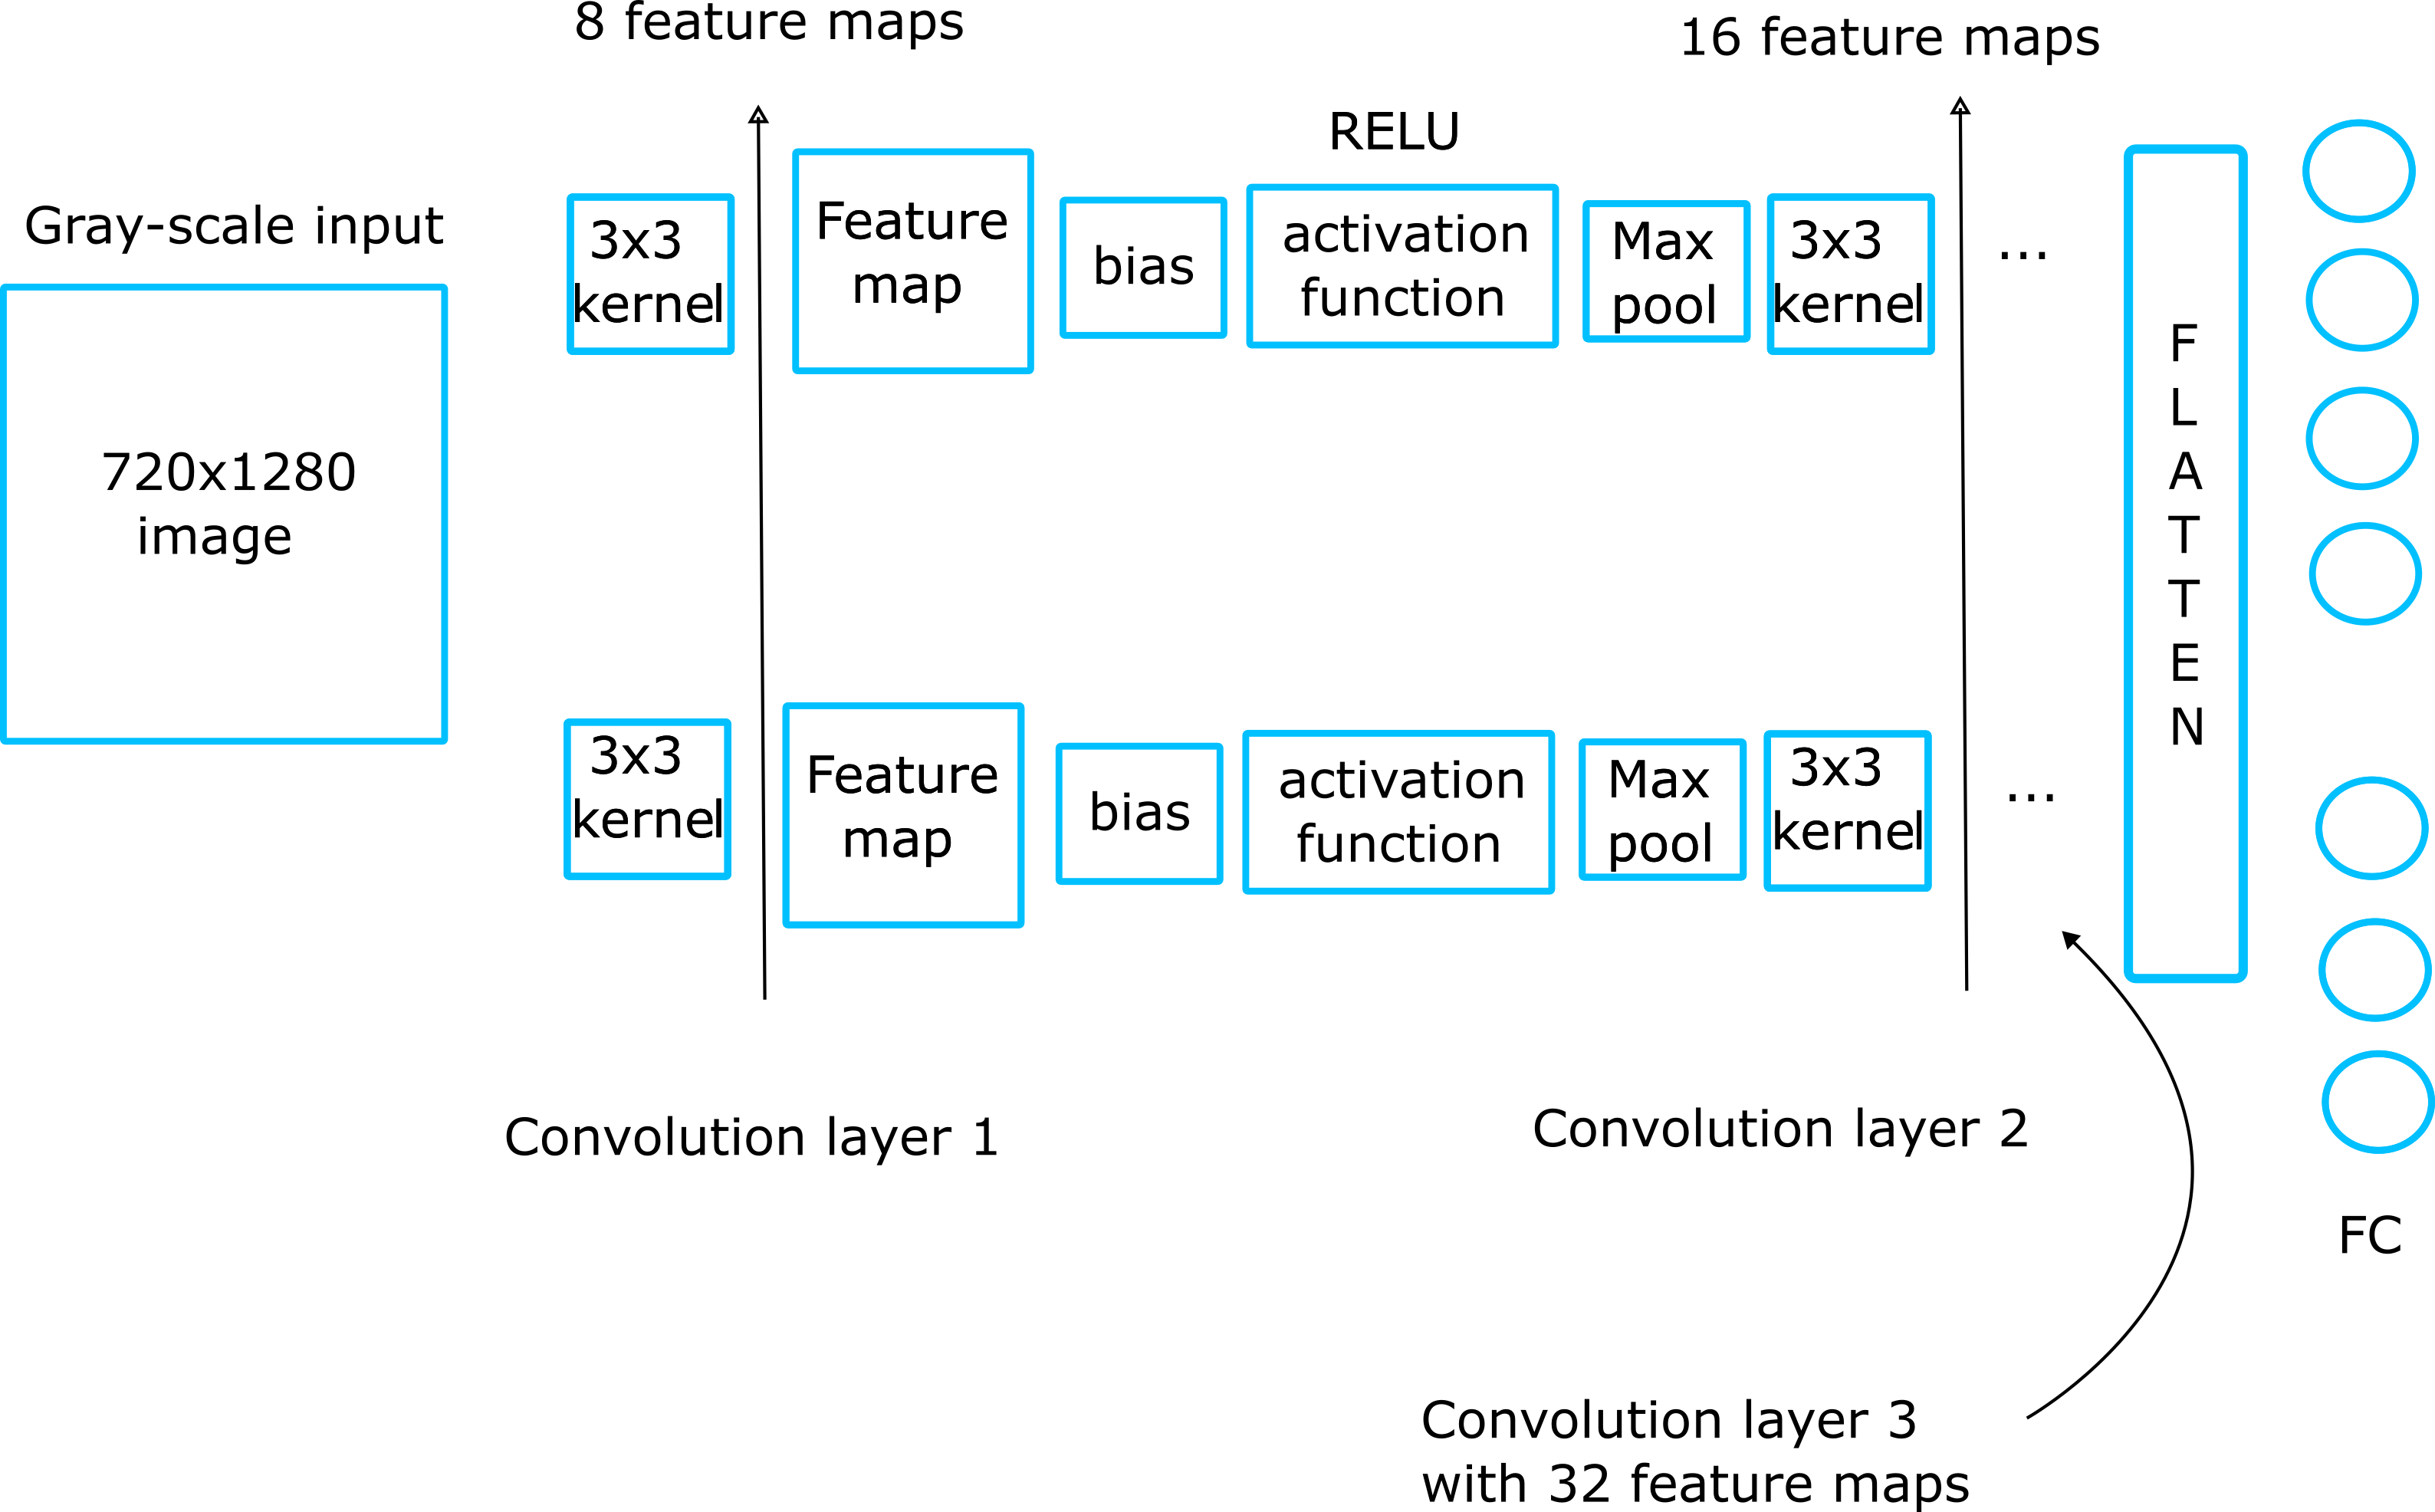
\includegraphics[width=0.5\textwidth]{graphics/cnn.png}
    \caption{Convolutional neural network architecture}
    \label{fig:arch}
    \end{figure}

    \begin{figure}[ht!]
        \begin{subfigure}{.3\textwidth}
          \centering
          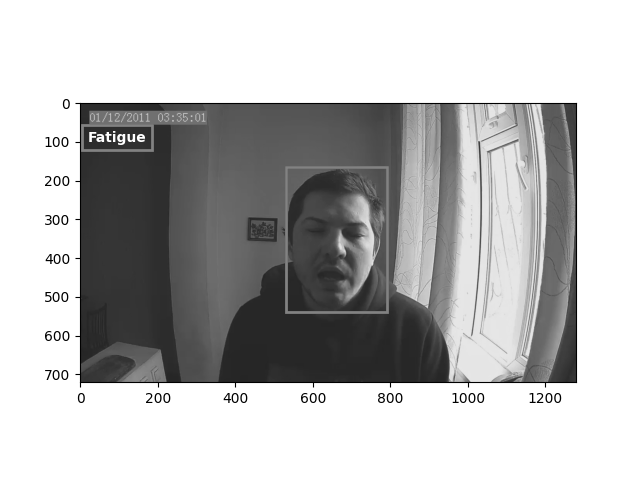
\includegraphics[width=.8\linewidth]{graphics/fatigue.png}
          \caption{Fatigue detection}
          \label{fig:sfig1}
        \end{subfigure}%
        \begin{subfigure}{.3\textwidth}
          \centering
          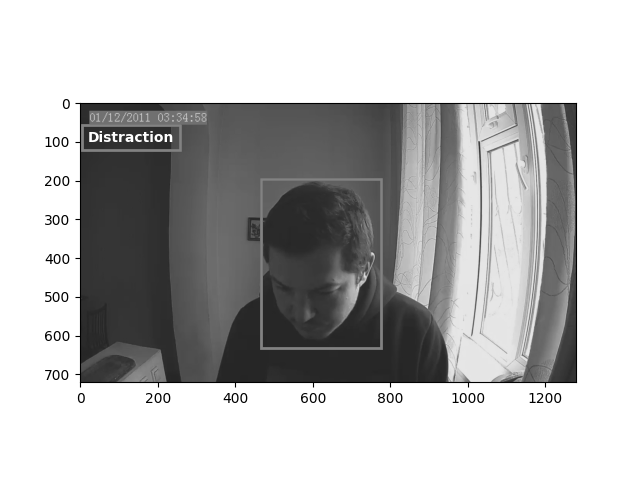
\includegraphics[width=.8\linewidth]{graphics/distraction.png}
          \caption{Distraction detection}
          \label{fig:sfig2}
        \end{subfigure}
        \begin{subfigure}{.3\textwidth}
            \centering
            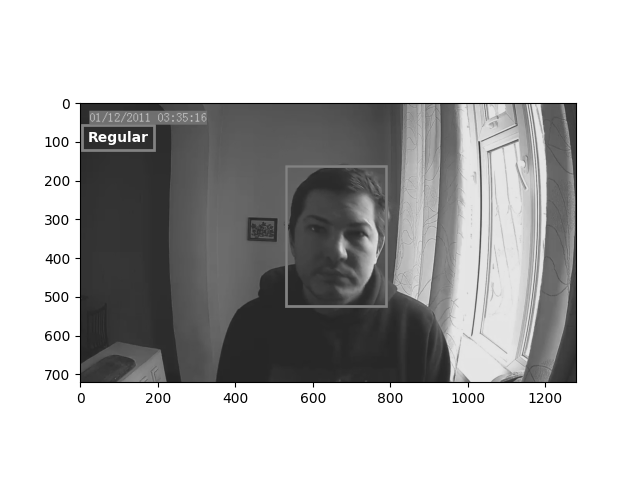
\includegraphics[width=.8\linewidth]{graphics/regular.png}
            \caption{Normal behavior}
            \label{fig:sfig2}
          \end{subfigure}
        \caption{Examples of different events}
        \label{fig:classification}
        \end{figure}



\section{Experimental results}
\label{section:results}
We have captured $1000$ images using a IR-capable camera, converted the images to
single channel images (gray-scale) and labeled $500$ images manually. That became 
our training dataset. Using these $500$ images we have trained the CNN, and then 
performed validation using remaining $500$ images. Finally, we have calculated the 
accuracy for our model: we have obtained $79.9\%$ accuracy on training dataset, 
which is rather good for such a small dataset (we assume that the weights of the 
CNN are updated on the backend once new labeled images become available). The examples 
of the classifications are shown in Figure1~\ref{fig:classification}. 


\section{Discussion}
\label{section:results}
We believe that there is a magnitude of application use cases for the developed 
prototype: from driving trucks in hazardous environments such as mine, to improving 
safety on regular roads. 

